\subsection{Análise de palavras das fontes de dados}

\subsubsection{Distribuição de palavras}

Assim como no tamanho dos documentos eu resolvi analisar para cada documento o percentual de palavras que não é verbo nem 
\textit{stopword} específica do contexto do trabalho. O gráfico abaixo mostra uma distribuição destes percentuais e podemos ver que a 
maioria está entre 40\% e 58\%, o que significa que após a remoção dos dois conjuntos de dados o tamanho destes documentos seriam 
reduzido para esta proporção. Felizmente vimos na análise gráfica dos tamanhos dos documentos que mesmo após o encurtamento os tamanhos
da maioria permanecia satisfatório.

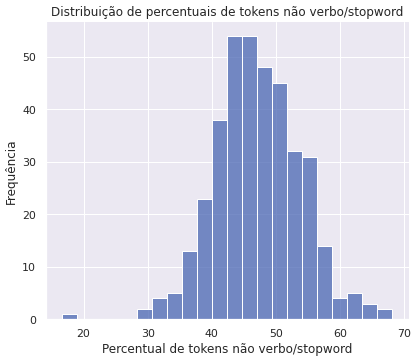
\includegraphics[scale=0.75]{explore/resources/analise_palavras_distribuicao_perc_nao_verbo_stopword.png}

\subsubsection{Análise estatística das fontes de palavras}

A primeira informação e mais simples é o total de palavras no dicionário. Percebe-se pelas informações abaixo que após a remoção de verbos 
e palavras específicas o dicionário caiu para 48\% de seu tamanho original.

\begin{itemize}
    \item Total de palavras: 114801
    \item Total de palavras após remoção de verbos e \textit{stopwords} específicas: 54862
\end{itemize}

A seguir eu procurei saber os 20 tokens mais frequentes do conjunto de dados. No conjunto original as 10 palavras que mais frequentes, 
assim como a quantidade de vezes que aparecem é:

\begin{lstlisting}
    [('fot', 1550), ('fic', 807), ('algum', 750), ('dia', 720), ('par', 660), ('caminh', 639), ('faz', 634), ('cheg', 611), ('pod', 599), ('visit', 581), ('fotograf', 566), ('passei', 560), ('parqu', 557), ('trilh', 554), ('outr', 551), ('bem', 538), ('cidad', 534), ('pass', 526), ('muit', 502), ('hor', 489)]
\end{lstlisting}

Após a remoção de verbos e algumas \textit{stopwords} específicas os 10 tokens mais frequentes são:

\begin{lstlisting}
    [('parqu', 557), ('cidad', 534), ('temp', 484), ('pouc', 422), ('lag', 364), ('jalap', 361), ('águ', 353), ('aind', 350), ('bonit', 348), ('vist', 338), ('bel', 322), ('pra', 297), ('lug', 297), ('fiz', 296), ('áre', 276), ('expos', 273), ('lad', 268), ('cacho', 253), ('pais', 246), ('qu', 245)]
\end{lstlisting}

\subsubsection{Nuvem de palavras}

Uma outra forma de informar visualmente as palavras mais frequentes no dicionário é uma nuvem de palavras. Abaixo vemos duas imagens.

A primeira ilustra o dicionário completo. Nota-se a predominância da palavras \textit{fot} e também dos verbos \textit{fic} e \textit{caminh}, removidos
ao fazer o treinamento. Na subseção anterior já tivemos a oportunidade de ver como estas palavras são predominantes.

\vspace{3mm} %3mm

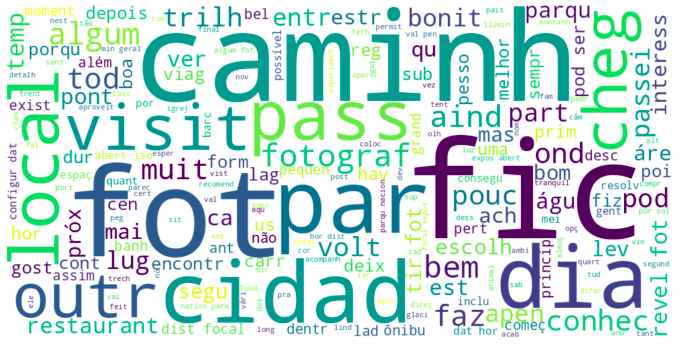
\includegraphics[scale=0.5]{explore/resources/nuvem_palavras_completo.png}

\vspace{3mm} %3mm

A segunda ilustra a frequência das palavras após a remoção de verbos e \textit{stopwords} específicas.

\vspace{3mm} %3mm

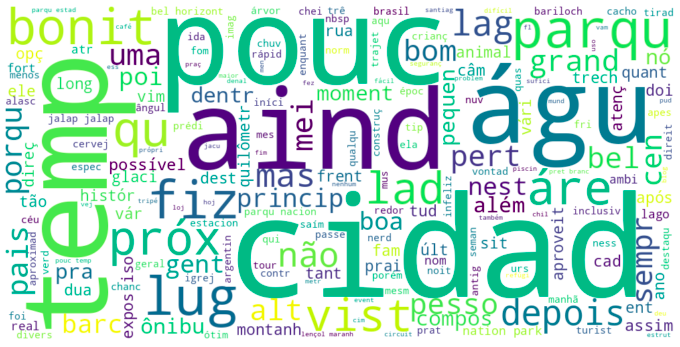
\includegraphics[scale=0.5]{explore/resources/nuvem_palavras_sem_verbos_sw.png}